Dataset manipulation and trimming of the dataset are two important techniques that can improve the predictions of an Feedforward Neural Network.
\subsection{Matrix}
We used a matrix representation (described in Section~\ref{sec:Matrix}) for the input parameters that were applicable for such a representation. The input (applicable for matrix) has to have a finite and limited set of values and a significant difference in how much the influence on the output differs between the input values. The inspiration for the matrix representation came from the way pictures are represented in ANNs. In \cite{knerr1992handwritten} they take every pixel (which has 16 different shades of grey) in a 16 pixel big image and map the pixels out as a matrix. This gives them 256 input variables for the ANN to represent this image. We do the same thing for the matrix applicable input parameters but instead of pixels we map out the different values e.g. the time of day where we can map every hour to a placeholder in the matrix.

The matrix format has limitations (as we saw in the wind power experiment two in Section~\ref{sec:windProdExperimentTwo}). The input parameters you want to represent as a matrix has to be evenly distributed in the dataset e.g. time of day, day of week etc. If this is not the case; some of the input values might be under trained(from under representation) and lead to errors in the predictions instead of improvements. This was the case with wind speed as a matrix and the reason to why it was worse than the wind speed as a single input variable. When we applied the matrix format to the time of day input variable we saw an improvement in both cases. We did a simple matrix test in the wind speed experiment two (Section~\ref{sec:windProdExperimentTwo}) as we only had two different parameters that were applicable for the matrix format and because we saw that the wind speed as a matrix did perform poorly. In the price experiments we did a more elaborate test of the matrix format and did every combination (all with matrix, all without matrix and mixed). We did these because the price experiments had more parameters that were representable on the matrix format thus giving us more combinations. The results from the price experiment was not as one-sided regarding the matrix format as the wind production experiments. In the price experiments we were not able to determine if one parameter had to be on one specific format. Mainly because the best combinations of the inputs contained both matrix and non-matrix formats --- we saw that the matrix format was overrepresented in the top results --- from which we can conclude that the matrix format in most cases helped the system perform better.

We have only seen one other paper use the matrix format (to some extend) for their seasonal inputs \cite{crowley2005weather}. They represented their days in the week as a matrix but they do not argue why they did it like that. The following articles has seasonal inputs but do not utilize the matrix format \cite{szkuta1999electricity, singhal2011electricity}. We highly anticipate that the predictions done in those papers could benefit from representing the seasonal inputs as a matrix. 

\subsection{Trimming}
Trimming of the dataset is a technique to remove irregularities in the dataset. This can be done both for the highest values and the lowest values in the dataset. Trimming allows us to get a more standardized dataset but it comes at a cost. All the data that you remove from the dataset you will not be able to predict in the test dataset thus introducing limitations to the predictions. Therefore trimming always has to be weighed up against how much of the dataset you will not be able to predict after the trimming. If the irregularities are extreme and under-represented in the dataset then we will most likely not be able to predict these values (because of under-training towards these extremes). If this is the case the outliers just introduce errors and do not add benefits because we are unable to predict them anyways thus justifying the removal of these values.

\begin{figure}[H]
\centering
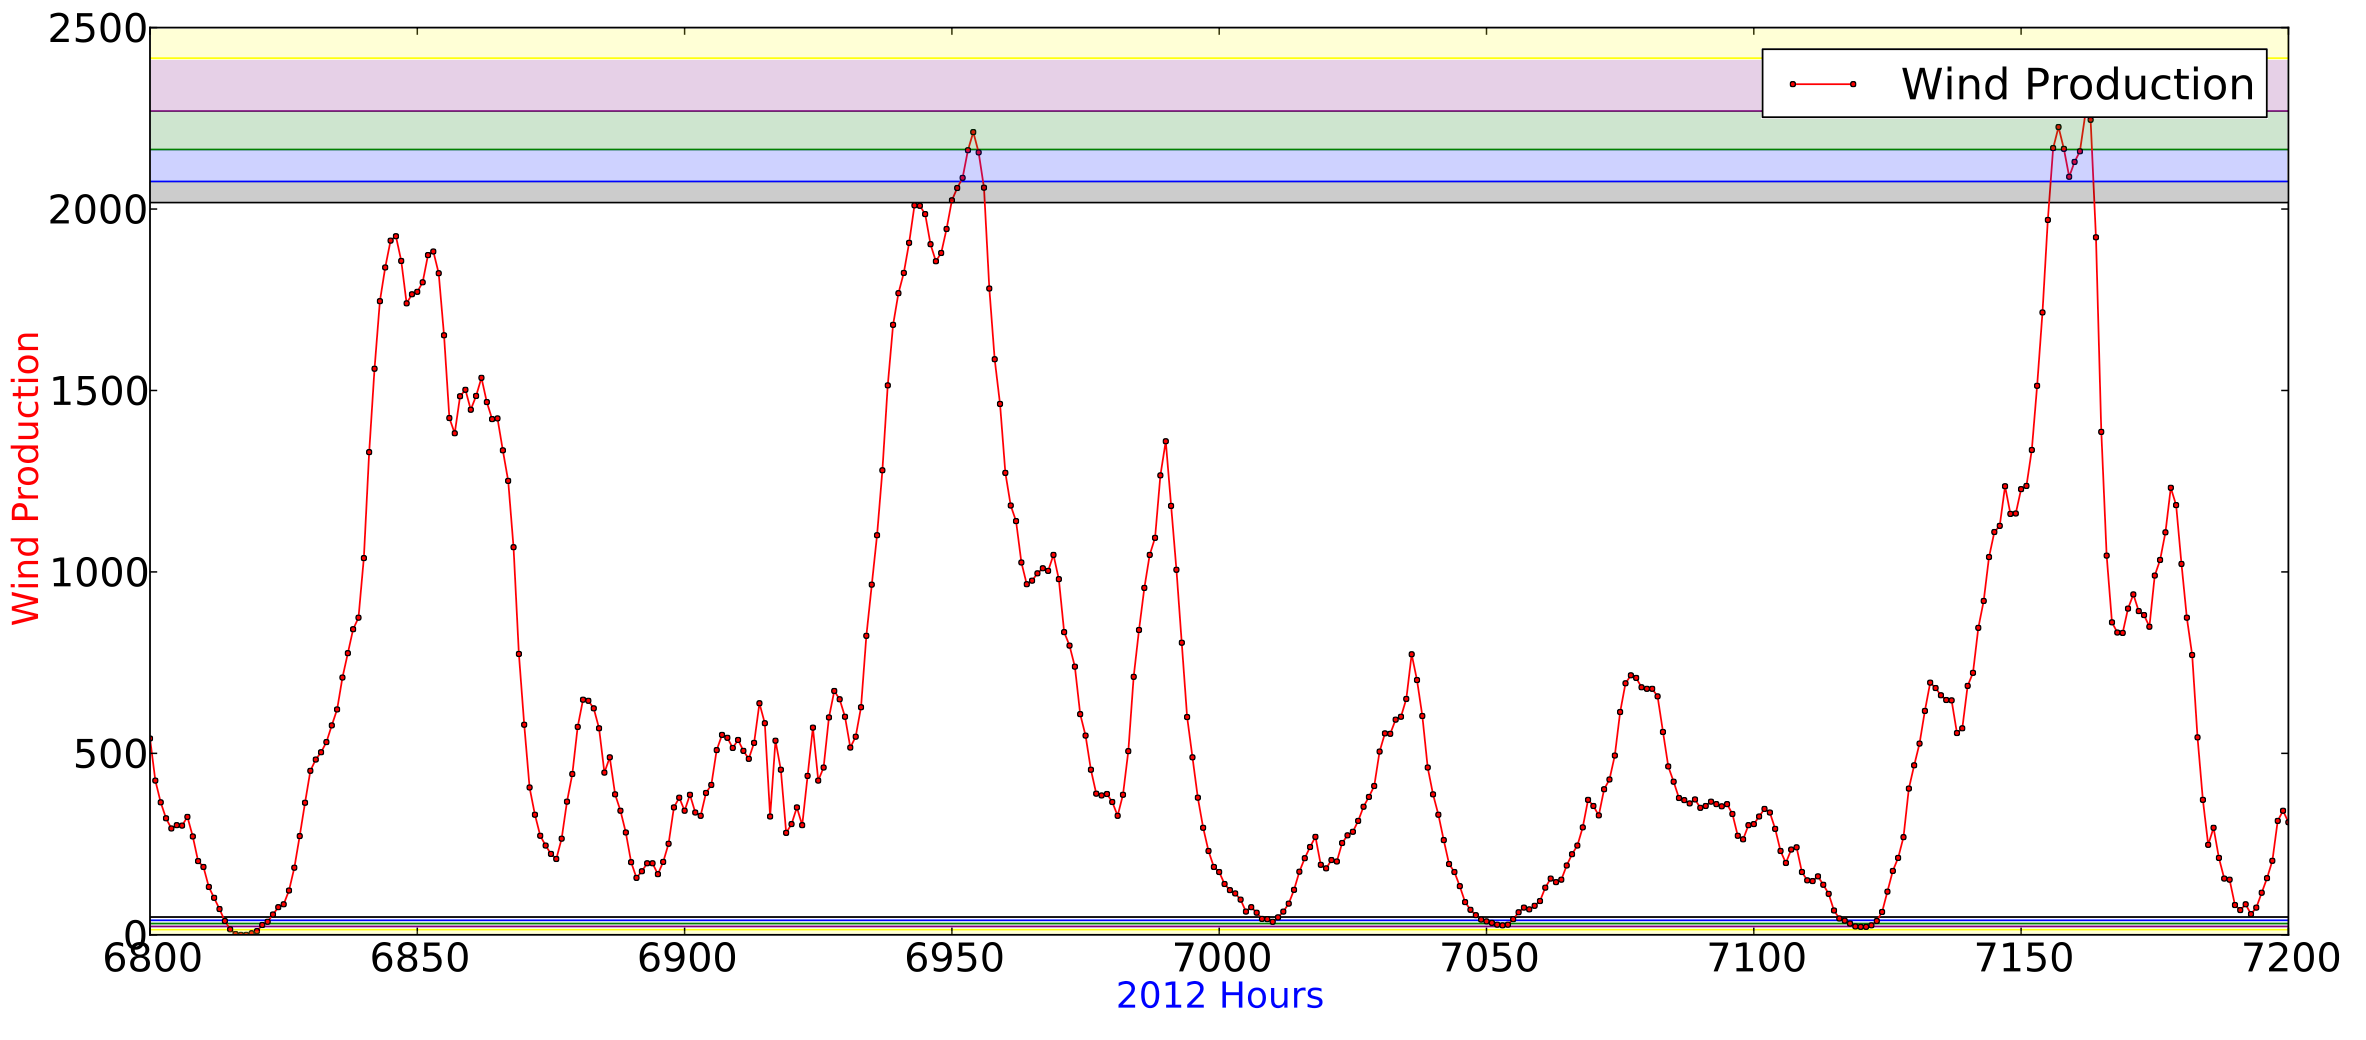
\includegraphics[width=0.99\linewidth]{billeder/pointingOutPlaceWhereTrim.png}
\caption{Trimming of the wind power production.}
\label{fig:pointingOutPlaceWhereTrimDataManipulation}
\end{figure}

In the wind power predictions experiment two (Section~\ref{sec:windProdExperimentTwo}) there were no benefit from trimming the dataset. Actually it introduced errors and made the predictions worse in average. This is because the dataset used for wind power production already consists of a uniform dataset and the trimming will only introduce more volatility as shown in Figure \ref{fig:pointingOutPlaceWhereTrimDataManipulation} because of this we will only focus on price in this section. In the electricity price prediction experiment two (Section~\ref{sec:priceExperimentTwo}) we saw that the trimming helped the predictions to become more accurate. This is because in the price prediction dataset there were some extreme outliers. When we trimmed the dataset by 1\% in the top we went from 1561 to 632 as the highest value in the dataset. The 1\% trim we did in the bottom of the dataset moved the minimum value from 0 to 61; this interval is not as steep as the one from the top --- but it contained price values of 0 which are special cases that we are not able to predict see Figure \ref{fig:1PTrimBottom} and therefore included in the trim. The 2\% we removed from the dataset when included in the dataset only introduced more noise to the predictions and no benefits thus removing them improved the performance i.e. it helped the remainder of the results to a better accuracy see Figure~\ref{fig:1PTrim}. We saw an improvement of 20,99\% from a non-trimmed dataset compared to a trimmed dataset (in the price predictions).

\begin{figure}[H]
\centering
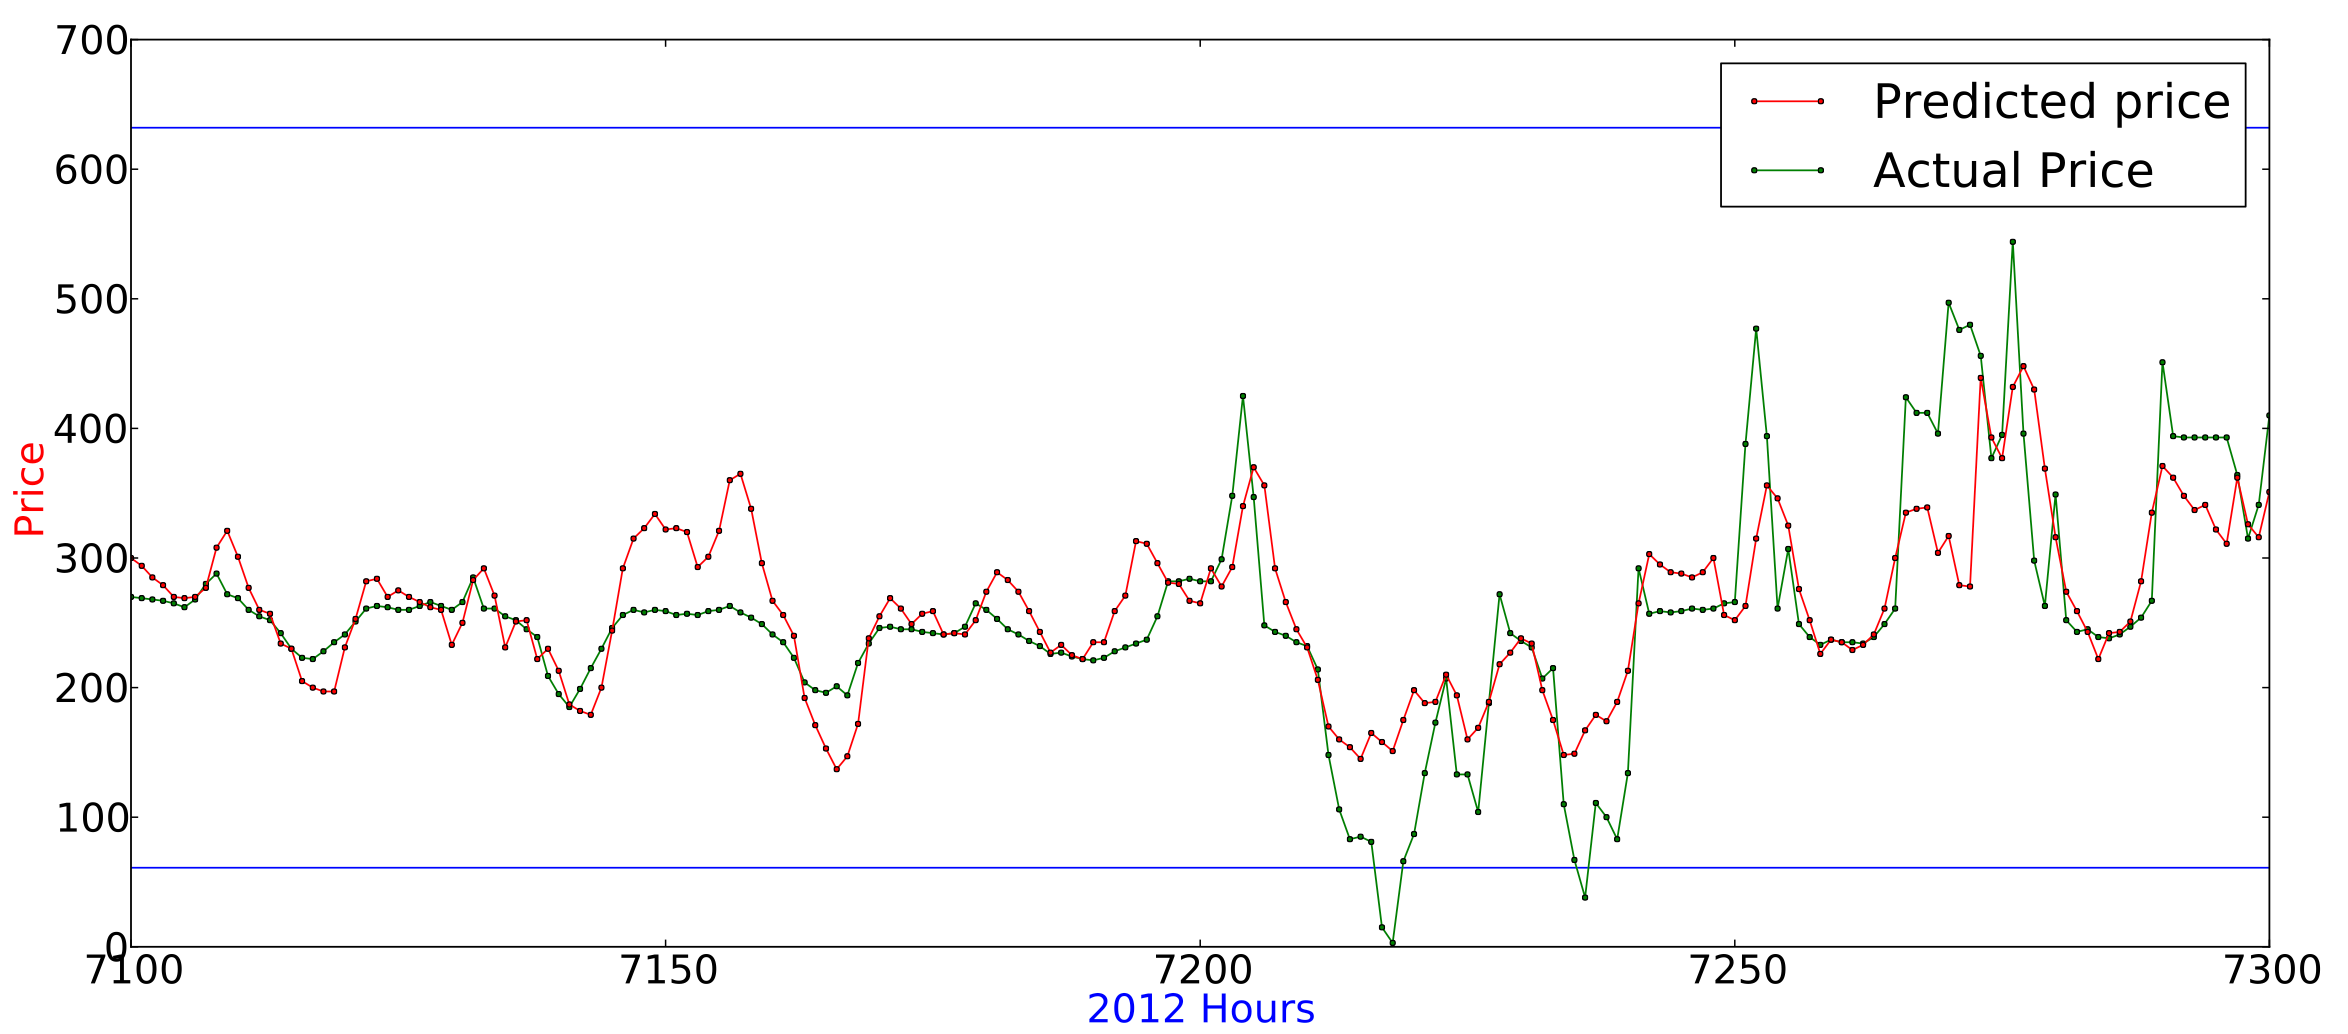
\includegraphics[width=0.99\linewidth]{billeder/Discussion/1PTrimBottom.png}
\caption{Electricity price forecast without trimming. The blue lines denote what would be removed by a 1\% top and bottom trim.}
\label{fig:1PTrimBottom}
\end{figure}

In \cite{singhal2011electricity, yamin2004adaptive} they also trim the dataset when predicting the electricity prices to get rid of the worst spikes in the price. They describe in details how they use trimming in their dataset. They use a form of trimming called \fnurl{Winsorising}{http://en.wikipedia.org/wiki/Winsorising} where they instead of removing the data they just set the values of the outliers to a specific value \cite{yamin2004adaptive}. In their case they set the upper value to \$50 and set every value that was above to \$50. The interesting part is that they introduce a post-processing scheme where they revert the winsorised values after the predictions thus not removing the high values from the set but just limiting the negative effects of the outliers. If this was done on our dataset we would see a decrease in performance\cite{yamin2004adaptive} but we would have a more accurate measure for how it would perform on live data. We see this as future work to test if this method will work on our dataset. Both matrix and trimming shows the need for preprocessing of the dataset also stated in \cite{yamin2004adaptive}. Preprocessing is important to increase accuracy and therefore very important to communicate to the reader of the paper due to the significant improvements in the performance. In \cite{sansom1999neural, 1} they do not mention anything about spike prices or whether they account for it. This might be because their dataset does not contain any spikes which (especially in large datasets) seems implausible see Section \ref{sec:volatility}. Which means we would have a hard time recreating their experiments --- since it seems like information has been omitted --- to see how well it performs on our dataset.

Another obstacle when talking about trimming is how it can be applied on a live dataset. Since we do not know what the price is for the next 24 hours we will not be able to include that in our calculations regarding what should be trimmed and what should not. If we chose to apply trimming we can only do those calculations on the training set. As mentioned earlier this makes us unable to reproduce the values that has been removed from the dataset. If the system was to be used in a real live setting as a decision support system the aforementioned limitations and what is written in \ref{sec:uncertainInformation} about uncertain information really emphasizes how important transparency is. We need to make the user aware of the limitations and benefits of trimming thus giving them an informed choice to make i.e. whether they benefit from applying trimming or not when predicting the next 24 hours.